The availability of static polymorphism in C++ leads to new ways of implementing classic design patterns. Take, for example, the Bridge pattern, which plays a major role in many C++ programs. One goal of using the Bridge pattern is to switch between different implementations of an interface.

\begin{center}
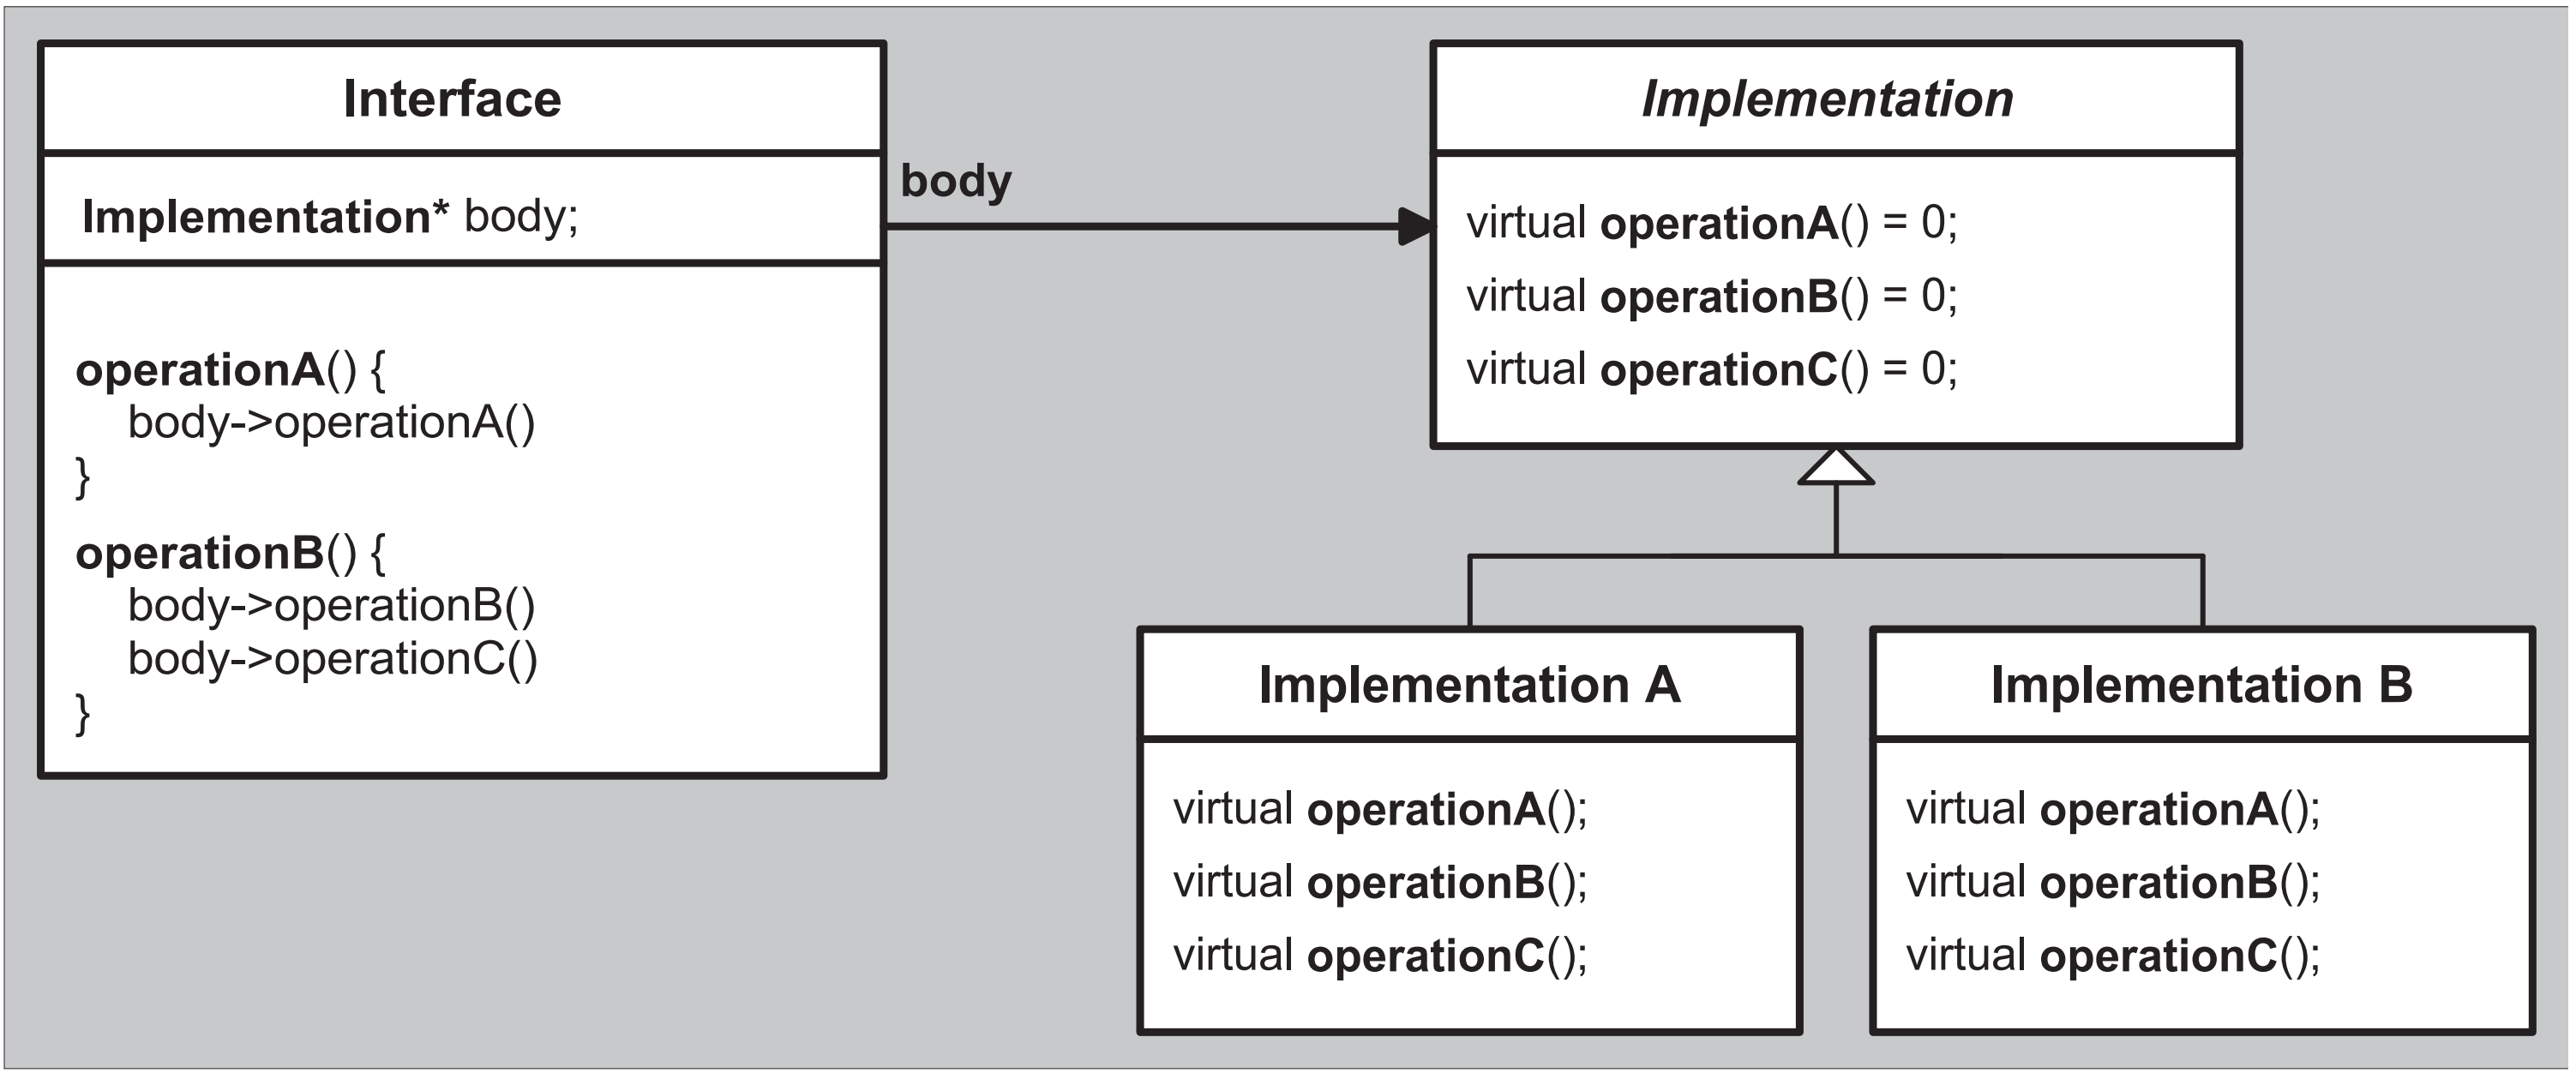
\includegraphics[width=0.8\textwidth]{content/3/chapter18/images/3.png} \\
Figure 18.3. Bridge pattern implemented using inheritance
\end{center}

According to [DesignPatternsGoF], this is usually done using an interface class that embeds a pointer to refer to the actual implementation and delegating all calls through this pointer (see Figure 18.3).

However, if the type of the implementation is known at compile time, we exploit the power of templates instead (see Figure 18.4). This leads to more type safety (in part, by avoiding pointer conversions) and better performance.

\begin{center}
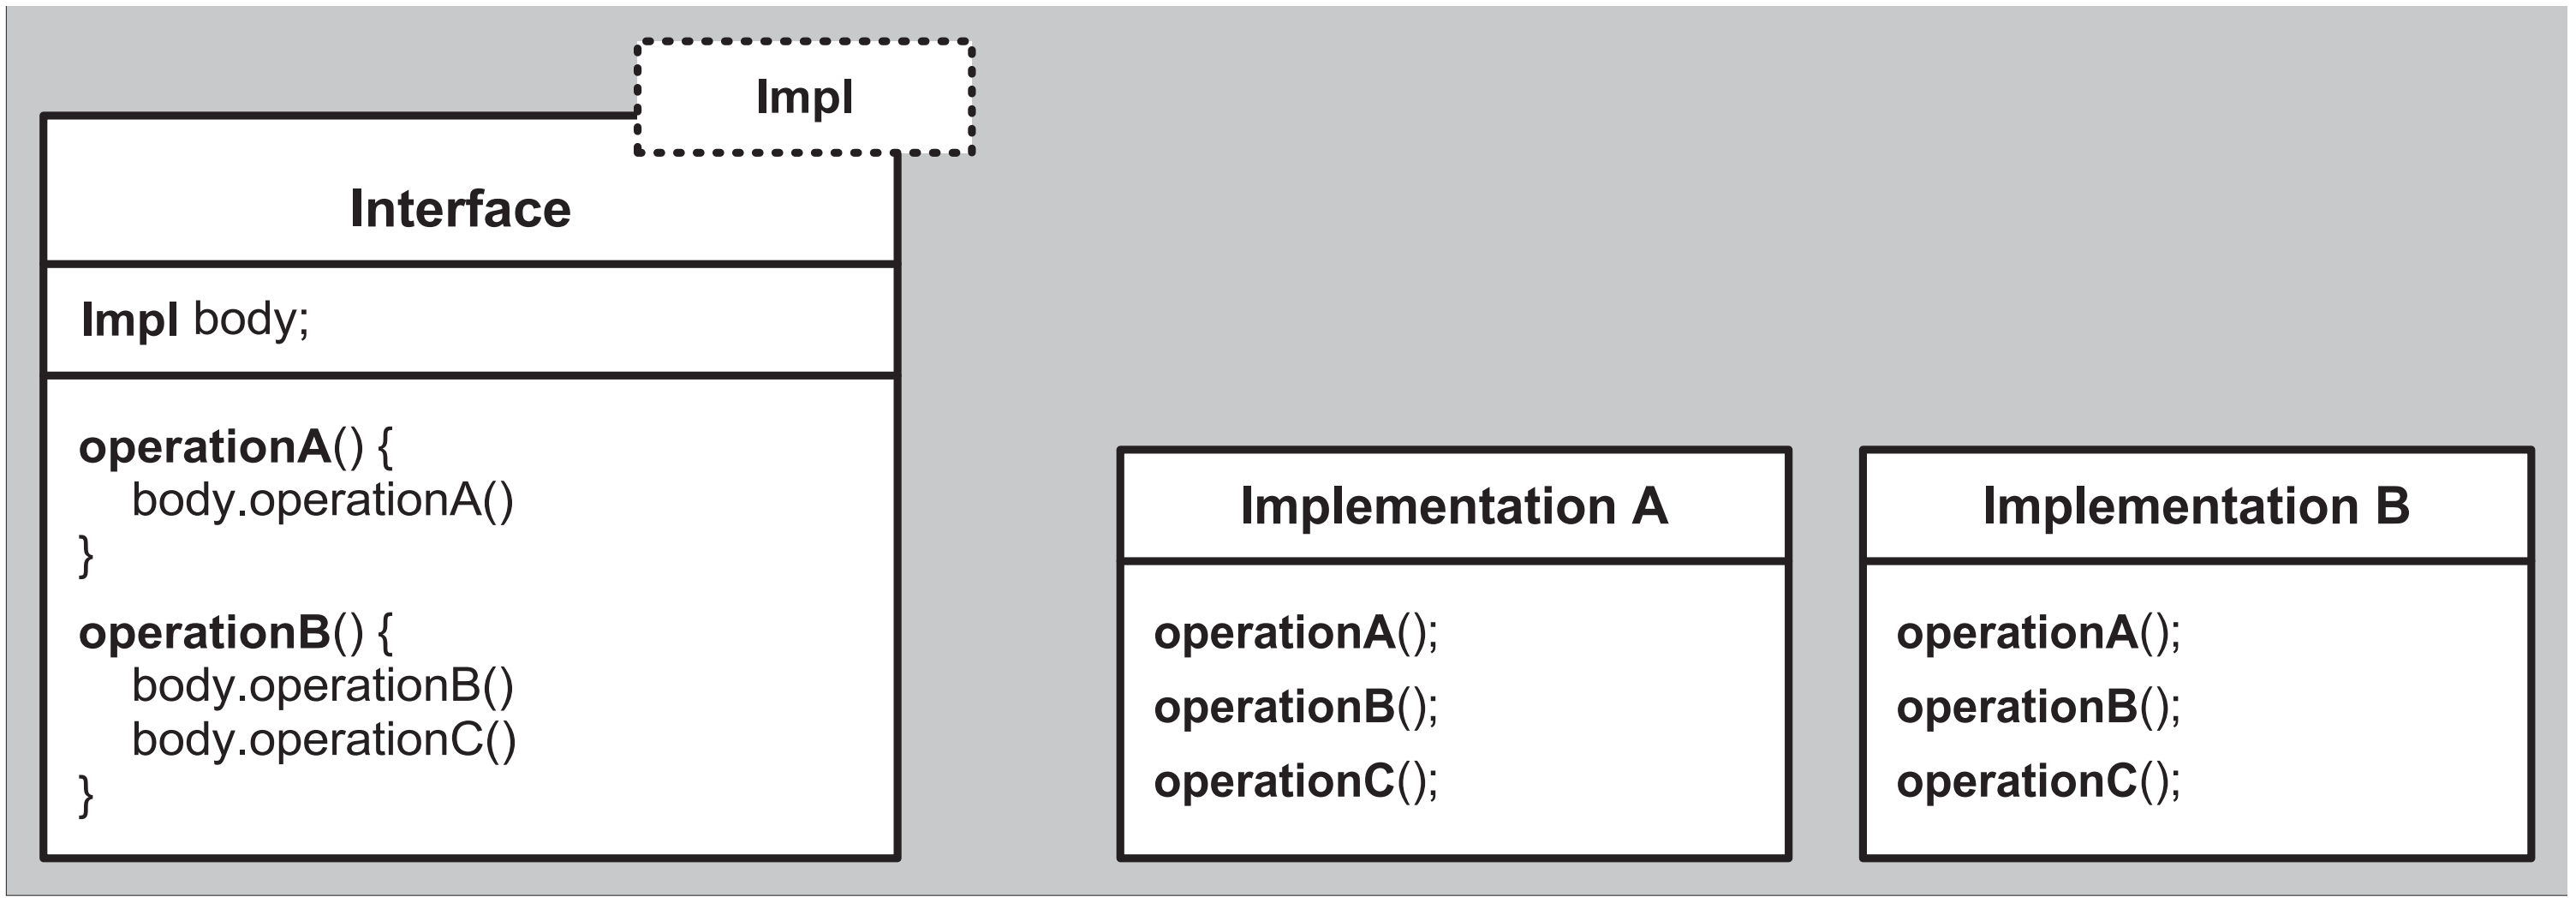
\includegraphics[width=0.8\textwidth]{content/3/chapter18/images/4.png} \\
Figure 18.4. Bridge pattern implemented using templates
\end{center}










































